\documentclass[12pt,letterpaper]{article}
\usepackage[utf8]{inputenc}
\usepackage{amsmath}
\usepackage{amsfonts}
\usepackage{amssymb}
\usepackage{graphicx}
\author{Jeffrey Wubbenhorst}
\title{Chapter 3}
\begin{document}

\maketitle

\begin{itemize}

% 3.1
\item Scalars have only magnitude. Vectors have both magnitude and direction. 

\item Two vectors $\vec{a}$ and $\vec{b}$ may be added geometrically by drawing them to a common scale and placing them head to tail. The vector connecting the tail of the first to the head of the second is the vector sum $\vec{s}$. Vector addition is commutative and obeys the associative law. 

\item The components of a a two-dimensional vector $\vec{a}$ are given as $a_x=\cos \theta \mbox{ and } a_y=a\sin \theta$ 

\item Magnitude and orientation of a vector are given as $a=\sqrt{a_x^2+a_y^2} \mbox{ and } \tan \theta=\frac{a_y}{a_x}$

% 3.2 
\item Unit vectors $\hat{i},\hat{j},\hat{k}$ have magnitudes of unity and are directed in the positive directions of the $x,y,\mbox{ and } x$ axes. Unit vectors are defined as $\hat{v}\equiv \frac{v}{|v|}$
% 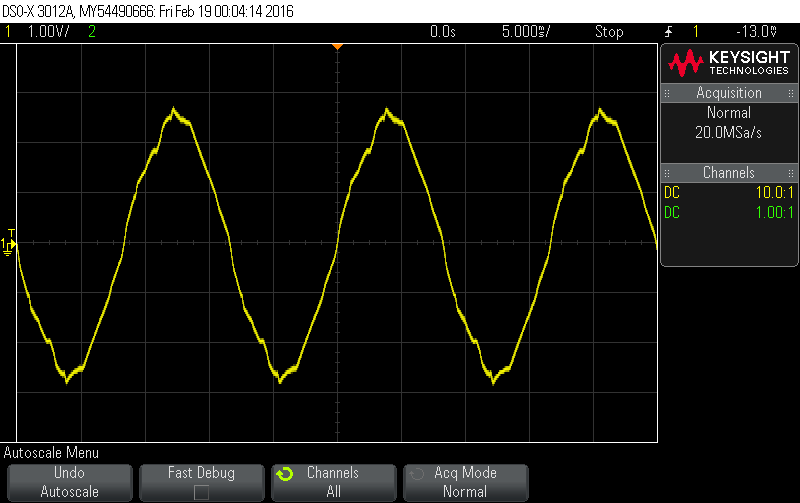
\includegraphics[scale=0.5]{scope_107.png}
% 3.3 

\item The scalar (or dot product) of two vectors $\vec{a} \mbox{ and } \vec{b}$ is written $\vec{a} \dot \vec{b}$ and is the scalar quantity given by $ab\cos \theta$ where $\theta$ is the angle between the directions of $\vec{a} \mbox{ and } \vec{b}$. 
\item The vector (or cross) product of two vectors is a vector whose magnitude is given as $c=ab\sin\theta$. The rest of it is ugly and we do not care. 

%$\vec{a}\times \vec{b}=/


\item 


\end{itemize}
\end{document}